\chapter{Displacement Mapping}
Surface details can be classified into microstructures, mesostructures and macrostructures. Microstructure are minute details, which is invisible to the human eye, so instead of being explicitly represented, its light scattering properties are typically modeled using \textit{bi-directional reflectance distribution functions (BRDFs)}. And macrostructure surfaces are designed by modelling, usually meshes, triangles, etc.

\begin{figure}\label{f:surface-details}
	\begin{subfigure}[t]{0.17\textwidth}
		\includegraphics[width=1.0\textwidth]{graphics/df/meso-structure-1}
		\caption{Sponge}
	\end{subfigure}
	\begin{subfigure}[t]{.285\textwidth}
		\includegraphics[width=1.0\textwidth]{graphics/df/meso-structure-2}
		\caption{Cloth}
	\end{subfigure}
	\begin{subfigure}[t]{.23\textwidth}
		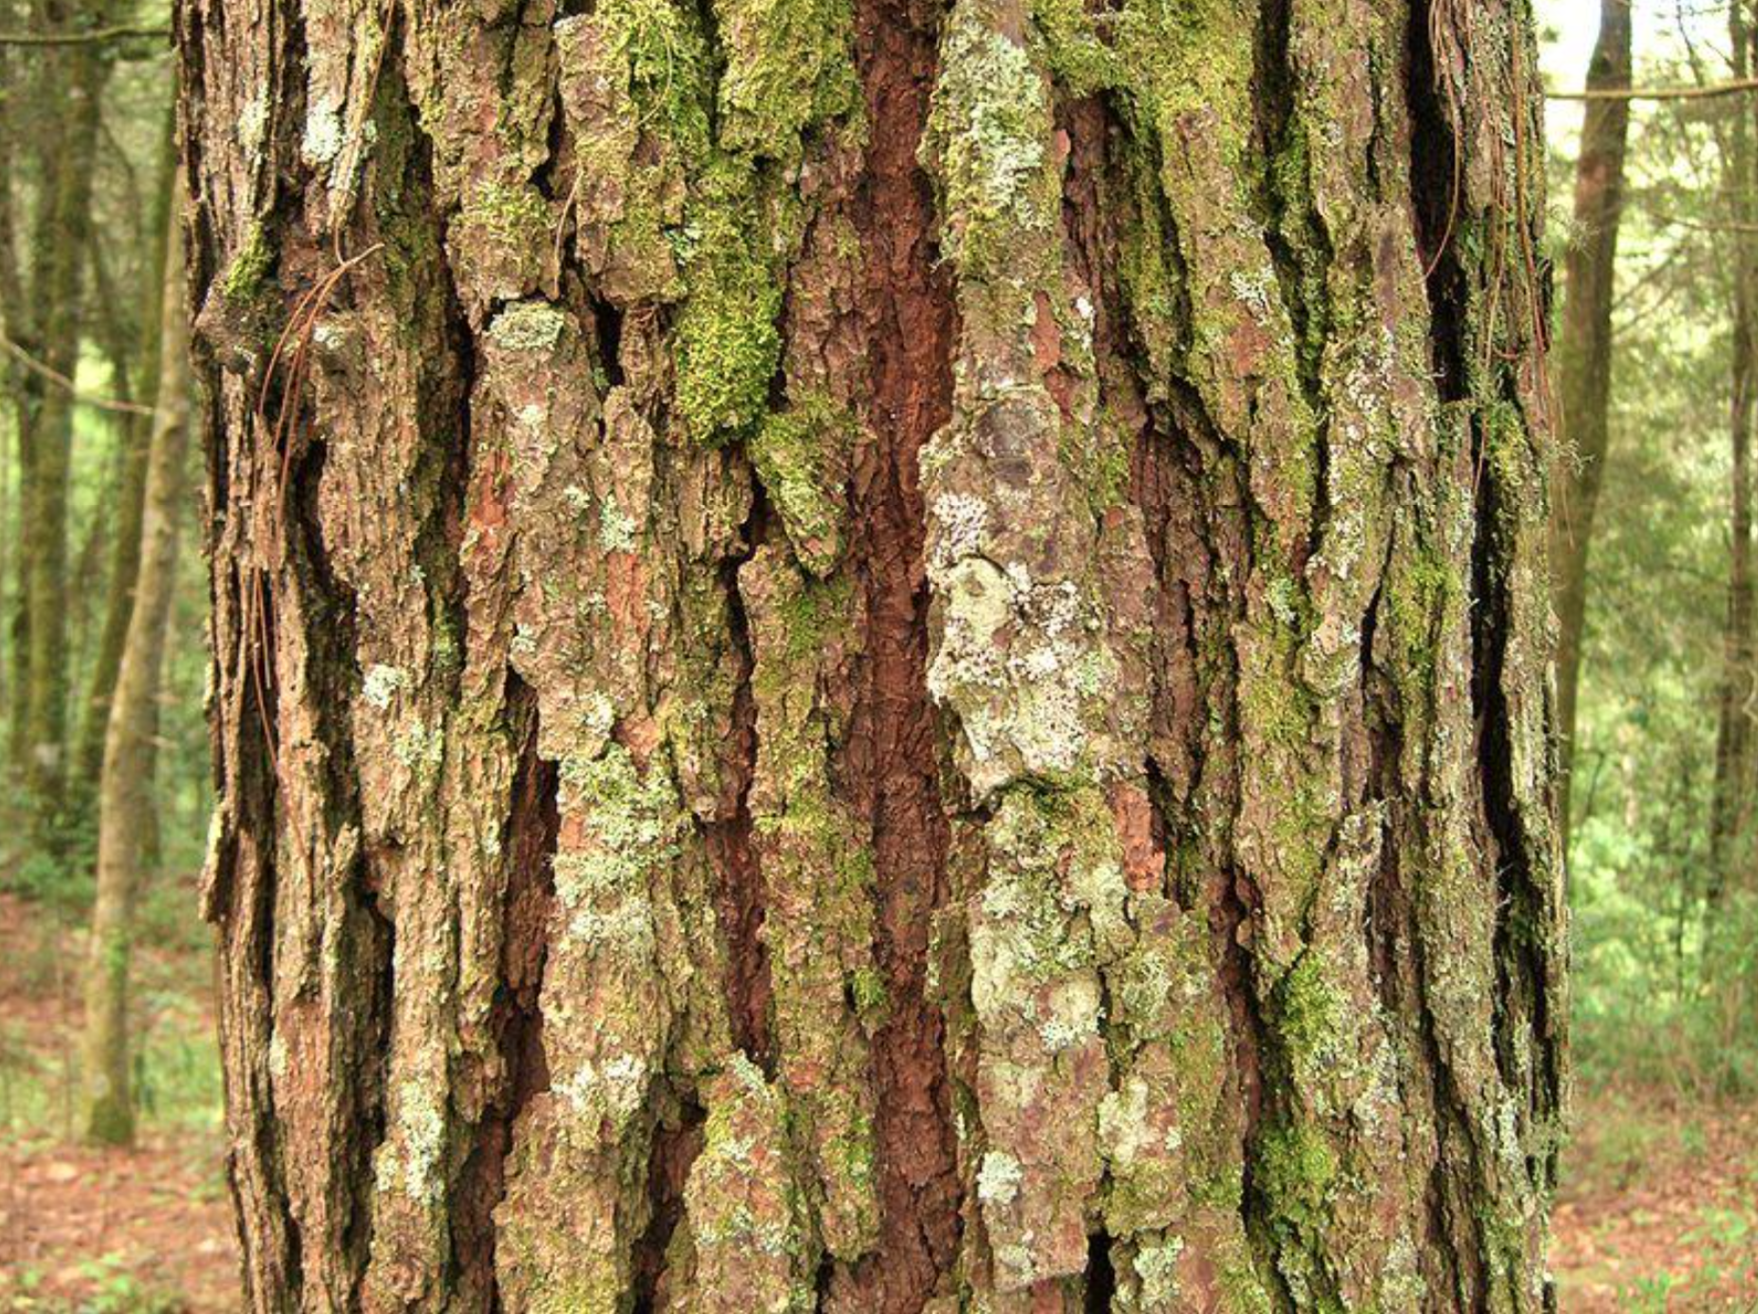
\includegraphics[width=1.0\textwidth]{graphics/df/meso-structure-3}
		\caption{Tree}
	\end{subfigure}
	\begin{subfigure}[t]{.26\textwidth}
		\includegraphics[width=1.0\textwidth]{graphics/df/meso-structure-4}
		\caption{Bread}
	\end{subfigure}
	\caption{Examples of volumetric mesostructures that are difficult to represent accurately with current interactive rendering techniques.}
\end{figure}

Mesostructures, see figure \ref{f:surface-details}, are fine-scale geometric details on the surface, and are large than microstructure but smaller than macrostructures. They are geometric which means we can handle it by computer graphics way, but it's hard to model it by meshes and triangles. They can significantly alter shadows, occlusion, and silhouettes. Displacement mapping techniques are usually used for mesostructures.



\section{What is Displacement Mapping}
To add small-scale to surfaces, Cook introduced displacement mapping in 1984\cite[-17mm]{a:Shade-Trees}. Unlike bump mapping, was introduced by Blinn in 1979\cite[-12mm]{a:SimulationofWrinkledSurfaces}, affects only the shading of surfaces, displacement mapping adjusts the positions of surface elements. Although parallax mapping, was introduced by Tomomichi Kaneko et al., in 2001\cite[-7mm]{a:DetailedShapeRepresentationwithParallaxMapping}, which also can displace the texture coordinates by a function of the view angle in tangent space and the value of the height map, it is a single step process that does not account for occlusion. Displacement mapping technique can alter shadows, occlusion, and silhouettes.

There are usually two implementations of displacement mapping. One is iteratively tessellates a base surface, pushing vertices along the normal of the base surface, and continuing until the polygons generated are close to the size of a single pixel. This method relies on the hardware support, such as the DirectX 11 tessellation which provides the ability to alert vertices in tessellation stage, it has never really caught on until recently. By this method, we usually use a vertex shader, Michael Bunnell presents this approach in \cite{a:AdaptiveTessellationofSubdivisionSurfaceswithDisplacementMapping}. Tessellation algorithm asks, "For this piece of geometry, what pixel in the image dose it map?"

Another has been long discussed is a ray tracing way, which do not rely on tessellation. This approach computes the real coordinates by ray tracing a hight-field or a 3D volume texture from the view ray in the pixel shader. This is the way we will talk about in this section. Contrast to tessellation, pixel shader is fast than vertex shader, and pixel shaders are better equipped to access textures. Moreover, by using pixel shader there is no need to generate the expensive intermediate vertices, so it saves memory. Ray tracing algorithm asks, "For this pixel in the image, what piece of geometry do we see?"

Lots of different methods which use ray tracing have been proposed. We mainly focus on the methods which using distance field to represent the displacement. Surprisingly, they quite efficient and have a high quality. 


\section{Relief Mapping (on a Plane)}
The first method we are discussing which focuses on a planar object. This method does not use a distance field texture presentation. It appeared firstly to introduce the basics of using ray tracing on displacement mapping.  

Fabio Policarpo et al, proposed a \textit{relief mapping} technique in 2005\cite{a:Real-TimeReliefMappingonArbitraryPolygonalSurfaces} based on an effifient ray-hight-field intersection algorithm implemented on the GPU. The technique uses a 2D hight-field texture and can be applied to polygonal representations. They are also improved this technique to apply it to no-hight-field \cite{a:ReliefMappingofNo-Height-FieldSurfaceDetails} surface in the next year. 

Figure \ref{relief-mapping-representation} shows a relief texture represented by its corresponding depth and normal maps. The depth map is quantized and represented using the alpha channel of the $RGB\alpha$ texture used to store the normal map. This way, a single 32-bit texel texture suffices to represent the structure of a relief texture.

The process of mapping relief data to a polygonal surface can be conceptually understand as following. For each fragment to be rendered:

\begin{figure}
\begin{center}
	\begin{subfigure}[c]{0.48\textwidth}
		\includegraphics[width=1.0\textwidth]{graphics/df/relief-mapping-representation1}
	\end{subfigure}
	\begin{subfigure}[c]{.48\textwidth}
		\includegraphics[width=1.0\textwidth]{graphics/df/relief-mapping-representation2}
	\end{subfigure}
\end{center}
	\caption{A relief texture represented by a depth (top) and a normal map (bottom). The normals are mapped to the [0,1] range and stored as an RGB image. The hight values also are normalized to [0,1], from top to bottom, the depth values vary from 0.0 to 1.0.}
	\label{relief-mapping-representation}
\end{figure}

\begin{enumerate}
	\item Compute the viewing direction (VD) as the vector from viewer to the 3D position of the point on the polygonal surface and transform VD to the tangent space. These steps formed a ray.
	\item Use VD and A, the $(s,t)$ texture coordinates of the fragment, to compute B, the $(u,v)$ texture coordinates where the ray reaches the depth value 1.0.
	\item Compute the intersection between VD and the hight-field surface using a binary search starting with A and B.
	\item Use the computed intersection point as the real texture coordinates to shade this fragment.
\end{enumerate}

The process is illustrated in figure \ref{f:relief-mapping}(a). They found that eight steps of binary subdivision is sufficient to produce very satisfactory results. This is equivalent to subdivided the depth range of the height field in $2^{8}=256$ equally spaced intervals. This approach also takes advantage of texture interpolation. As the depth map is treated and accessed as a texture, texture filtering ($e.g.$, bilinear) guarantees that the height-field surface will be continuous.

The binary search procedure just described may lead to incorrect results if the viewing ray intersects the height field surfaces in more than one point, as illustrated in figure \ref{f:relief-mapping}(b).

\begin{figure*}\label{f:relief-mapping}
	\begin{subfigure}[t]{0.33\textwidth}
		\includegraphics[width=1.0\textwidth]{graphics/df/relief-mapping1}
		\caption{Binary search}
	\end{subfigure}
	\begin{subfigure}[t]{.33\textwidth}
		\includegraphics[width=1.0\textwidth]{graphics/df/relief-mapping2}
		\caption{Incorrect}
	\end{subfigure}
	\begin{subfigure}[t]{.33\textwidth}
		\includegraphics[width=1.0\textwidth]{graphics/df/relief-mapping3}
		\caption{Linear search}
	\end{subfigure}
	\caption{The real process is first using linear search(c) to find the first point(\textcircled{3} in (c)) inside the surface. Then using binary search(a) starts from \textcircled{2} and \textcircled{3}.}
\end{figure*}

In order to avoid missing the first intersection, they start a linear search first and find the first point inside the surface; Once the first point under the height field surface has been identified, the binary search starts using the last point outside surface and current one. This process is very much like the traditionary ray marching process we have discussed before.

Using the similar process, we can compute the shadow ray intersection with the height field from the light.

Unfortunately, linear search requires a fixed step size. This means that in order to resolve small details, it is necessary to increase the number of steps, forcing the user to trade accuracy for performance.


\section{Per-pixel DP with Distance Functions}
Based on relief mapping technique, William Donnelly proposed a method in 2005\cite{a:Per-PixelDisplacementMappingwithDistanceFunctions} which uses a distance field instead of the height-field, so it can use sphere tracing automatically adjusts the step size as necessary to provide fine detail near the surface, while skipping large areas of empty space away from the surface.

To generate the distance field texture, the algorithm first create a 3D map where each pixel stores a 3D displacement vector to the nearest point on the surface, then performs a small number of sequential sweeps over the 3D domain, updating each pixel's displacement vector based on neighbouring displacement vectors. This is the distance transform algorithm we have introduced before. Once the displacement have been calculated, the distance for each pixel is computed as the magnitude of the displacement.

\begin{figure}
\sidecaption
	\includegraphics[width=0.65\textwidth]{graphics/df/08_displacement_06}
	\caption{Generated by distance maps way.}
\end{figure}

We then could use sphere tracing to compute the ray intersection with the distance field surface, which is faster than the combination of linear and binary search introduced by relief mapping. 

All the other things are same as relief mapping technique. The view ray was transformed to the tangent space. Then use sphere tracing, instead of linear and binary search, to compute the intersection point, the value of which in the distance field will be used as the real coordinates.

They experimented with maps up to $512\times512\times32$ (all examples in that paper they use ($512\times512\times16$) for complex data sets. They set the value of NUM\_ITERATIONS to 16 iterations for our examples. In most cases, this was more than sufficient, with 8 iterations sufficing for smoother data sets.

But the memory requirement for volumetric textures is high and sampling frequency must be carefully chosen to ensure high rendering quality. In the following sections we will introduce some improved approach called directional distance maps.

\section{Shell Maps}
So far, we've introduced the basics of displacement mapping using ray tracing and we focused on planar surface. It's time to go further. This section is very important, we will discuss two basically theories: How represent arbitrary surfaces and how to handle the coming along problem: texture distortion?

Although most textured surface representations work well for objects of simple topology, they are not practical for representing objects with fine-scale geometric detail. It is necessary to address volumetric methods for textures, which require a three-dimensional parameterization. 

\begin{figure}\label{f:shell-space}
	\begin{center}
		\includegraphics[width=0.65\textwidth]{graphics/df/shell-maps-1}	
	\end{center}	
	\caption{Shell space is the region between a base surface and an offset surface to the base. A shell map is a one-to-one function between texture space and shell space.}
\end{figure}

\textit{Shell space}\cite{a:Shell-Maps}, which has been proposed by Serban D. Porumbescu et al, can be defined as a bounded region between the \textit{base surface} $S$ and a constructed \textit{offset surface} $S_{o}$. A \textit{shell map} is a bijective mapping between shell space and texture space, as shown in figure \ref{f:shell-space}. By using shell space and shell map, we can use a thick three-dimensional volume texture to represent a surface with fine-scale geometric detail. Just like the 2D texture can be mapped to a normal meshes.

The last section only applies distance mapping to planes. By using shell maps, this method can be applied to general meshes. Every single triangle in $S$ is extruded toward its normal and form a prism volume in shell space. Each prism has a corresponding prism in texture, generated by using the texture coordinates of the vertices of the shell-space, see figure \ref{f:prisms}.

\begin{figure}\label{f:prisms}
	\begin{center}
		\includegraphics[width=0.9\textwidth]{graphics/df/shell-maps-2}	
	\end{center}	
	\caption{Prisms in shell space correspond to prisms in texture space.}
\end{figure}

For offset surface generation, they adopted Cohen's algorithm\cite[-19mm]{a:SimplificationEnvelopes}. First, $S_{o}$ is generated by duplicating $S$. This establishes the basic correspondence between triangles and vertices in the two meshes. The vertices of $S_{o}$  are assigned the same texture coordinates as the corresponding vertices of $S$ . Each vertex $\mathbf{v}$ of $S$ is assigned a "direction" vector $\vec{d}$, which is a linear combination of the normal vectors of the triangles of which $\mathbf{v}$ is a vertex. So is then displaced away from $S$ by iteratively moving vertices $\mathbf{v}_{o}$ of $S_{o}$ along the direction vectors associated with the corresponding vertex $\mathbf{v}$ of $S$. Please see the paper for additional details. 

For fine-surface detail a "constant-distance" offset surface is best to keep the detail consistent over the surface. Arbitrary offset surface can be manually constructed but it must satisfy two properties, or it may will generate distortion:

\begin{itemize}
	\item $S$ and $S_{o}$ must have the same number of triangles and the same mesh connectivity. Each triangle $\tau\in S$ must be associated with a unique triangle $\tau_{o}\in S_{o}$. Each vertex $\mathbf{v}\in S$ must be associated with a unique vertex $\mathbf{v}_{o}\in S_{o}$.
	\item $S_{o}$ should have no self intersections and should not intersection $S$.
\end{itemize}

\begin{figure}
\sidecaption
	\includegraphics[width=.65\textwidth]{graphics/df/shell-maps-3}		
	\caption{Prisms are split into three tetrahedra. Prisms can be split in six ways, depending on the direction of the triangulation of the quadrilateral faces. The six splits can be characterized with labels (FRR, RFR, RRF, RFF, FRF, and FFR) depending on the triangulation of the quadrilateral faces.}
	\label{f:tetrahedra}
\end{figure}

Texture-space prisms are right triangular prism, but shell-space prisms are generally non-convex. To create a robust mapping, they split the prisms into three tetrahedra by triangulating the three quadrilateral faces, see figure \ref{f:tetrahedra}. By splitting corresponding prisms $P$ and $P_{t}$ in the same way, we establish a correspondence between tetrahedra in shell space, and tetrahedra in texture space, where each tetrahedron $T$ in shell space has a unique corresponding tetrahedron $T_{t}$ in texture space.



Given a tetrahedron $T$ in shell space, and its corresponding tetrahedron $T_{t}$ in texture space, any point $\mathbf{p}$ in $T$ can be associated with a unique point $\mathbf{p}_{t}$ in $T_{t}$ using barycentric coordinates\footnote{If $\mathbf{v}_{1}$, $\mathbf{v}_{2}$, $\mathbf{v}_{3}$ and $\mathbf{v}_{4}$ are the vertices of a tetrahedron $T$, and $\mathbf{p}$ is a point in $T$, then the barycentric coordinates $(\alpha_{1},\alpha_{2},\alpha_{3},\alpha_{4})$ of $\mathbf{p}$ in $T$ are defined such that $\mathbf{p}= \alpha_{1}\mathbf{v}_{1} +\alpha_{2}\mathbf{v}_{2} +\alpha_{3}\mathbf{v}_{3} +\alpha_{4}\mathbf{v}_{4}$, where $\alpha_{1} +\alpha_{2} +\alpha_{3} +\alpha_{4} = 1$.}. That is, if $B(T,\mathbf{p})$ defines the barycentric coordinates of $\mathbf{p}$ in $T$, and $\phi(T,\alpha)$ defines the point in $T$ with barycentric coordinates $\alpha$, then

\begin{equation}
	\begin{split}
		\mathbf{p}_{t}&=\phi(T_{t},B(T,\mathbf{p})) \text{,  and} \\
		\mathbf{p}&=\phi(T,B(T_{t},\mathbf{p}_{t}))
	\end{split}
\end{equation}

establishing the bijective mapping between shell space and texture space.

Procedural and geometry textures can be rendered using ray tracing, in which rendering is accomplished by transforming world-space ray segments to texture space and by marching rays through texture space. But this will generate texture distortions, see figure \ref{f:ray-tracing-in-shell-space}, as a straight ray in shell space can be a piecewise segments in texture space. 

\begin{figure}\label{f:ray-tracing-in-shell-space}
	\begin{center}
		\includegraphics[width=0.8\textwidth]{graphics/df/shell-maps-5}	
	\end{center}	
	\caption{Rays intersect tetrahedra in shell space (a). Rays are marched in shell space, and points are transformed to texture space for density calculations. This method effec- tively traces curved rays through texture space (b).}
\end{figure}

To solve this problem, The ray should be marched in shell space, and points are be transformed to texture space density calculation and for ray-surface intersection calculation.

There are some clever methods, in which instead of marching along rays, techniques using high-dimensional texture functions do view-dependent texture lookups, effectively trading off runtime calculations with storage requirements. In the next two sections we will discuss these this kind of methods. 

But all of the these techniques exhibit artifacts under macrostructure deformation, since the precalculated visibility data are computed for a single mesh configuration.


\section{Generalized Displacement Maps}
In 2004, Xi Wang etc al, present a general mesostructure rendering technique\cite[-85mm]{a:GeneralizedDisplacementMaps} based on a proposed \textit{generalized displacement map (GDM)}, which represents the distance of solid mesostructure along any ray cast from any point within a volumetric texture. GDM provides a even faster approach to find intersection point due to it's special data structure. GDM also provides less texture distortion by computing mesostructure visibility jointly in object space and texture space.

\begin{figure}
\begin{center}
	\begin{subfigure}[b]{.48\textwidth}
		\includegraphics[width=1.0\textwidth]{graphics/df/GDM-model-1}	
		\caption{}
	\end{subfigure}
	\begin{subfigure}[b]{.48\textwidth}
		\includegraphics[width=1.0\textwidth]{graphics/df/GDM-model-2}	
		\caption{}
	\end{subfigure}
\end{center}	
\caption{GDM model. (a) The GDM for a ray cast from point $P$ in direction $V$ is defined as the distance of the nearest solid volume. (b) Three cases in GDM computation. From top to bottom: $P$ outside solid volume with an intersection in direction $V$, $P$ outside solid volume with no intersection in direction $V$, Plying within solid volume.}
\label{f:GDM-modelling}
\end{figure}

This method first takes mesostructure geometry as input and compute its GDM. After the GDM texture is mapped to a surface, rendering is performed by a per-pixel algorithm that can be accelerated in hardware.


As figure \ref{f:GDM-modelling} illustrated, from each point $p=(x,y,z)$ a ray is cast toward sampled viewing directions $\vec{V}=(\theta,\phi)$ expressed in spherical angles, where the polar angle $\theta$ ranges from 0 to $\pi$. The 5D GDM $d_{GDM}(x,y,z,\theta,\phi)$ records the distance along each viewing direction to the nearest mesostructure surface, according to

\begin{equation}
	d_{GDM}(x,y,z,\theta,\phi)=
	\begin{cases}
		d & \text{if ray intersects mesostructure}\\
		d_{max} & \text{if no intersection exist}\\
		0 & \text{if $p$ inside solid volume}
	\end{cases}
\end{equation}

The three different cases for this measurement are displayed in figure \ref{f:GDM-modelling}(b).

\begin{figure}\label{f:gdm-triangle-prism}
\begin{center}
	\begin{subfigure}[b]{0.4\textwidth}
		\includegraphics[width=1.0\textwidth]{graphics/df/GDM-object-space}	
		\caption{Object space}
	\end{subfigure}
	\begin{subfigure}[b]{0.4\textwidth}
		\includegraphics[width=1.0\textwidth]{graphics/df/GDM-texture-space}	
		\caption{Texture space}
	\end{subfigure}
\end{center}	
\caption{An extruded prism in object space, and its corre- sponding volume in texture space.}
\end{figure}

The GDM can then be mapped onto an arbitrary surface like a volumetric texture $V(x,y,z)$ with a 2D function of $(\theta,\phi)$ stored in each voxel. Mapping a volume texture onto a triangle mesh extrudes each triangle vertex towards its normal direction to generate a prism volume for each mesh triangle, as exemplified in figure \ref{f:gdm-triangle-prism}. Hence, the mesostructure of each prism in the object space is given by a corresponding volume in the texture space. The bilinear prism fins are each approximated by two mesh triangles. Each fin is shared by two prisms, and its normal directions are defined outwards with respect to the prism being processed.

\begin{figure}\label{f:gdm-rendering-ray}
\begin{center}
	\begin{subfigure}[b]{0.3\textwidth}
		\includegraphics[width=1.0\textwidth]{graphics/df/GDM-object-space-ray}	
		\caption{Object space}
	\end{subfigure}
	\begin{subfigure}[b]{0.3\textwidth}
		\includegraphics[width=1.0\textwidth]{graphics/df/GDM-texture-space-ray}	
		\caption{Texture space}
	\end{subfigure}
\end{center}	
\caption{Ray path in object space and its corresponding path in texture space.}
\end{figure}

In contract to methods for volumetric texture rendering, the GDM rendering algorithm does not trace rays through mesostructures synthesized onto a surface. Instead, it rapidly processes ray segments in each extruded prism in texture space, as illustrated in figure \ref{f:gdm-rendering-ray}.

But as mentioned above, this techniques exhibit artifacts under macrostructure deformation, since the precalculated visibility data are computed for a single mesh configuration. 

GDM has fast ray-surface intersection calculation since it precomputed the ray tracing calculation in a hight-dimensional texture,but which means more memory needed. The next section we will introduce a method which based on GDM but use less memory. 



\section{Directional Distance Maps}
Basically, GPU-based ray-object intersection algorithms employ two strategies. One attempts to bracket the intersection between two ray points and then searches for the root within this interval, such as the aforementioned \textit{relief mapping}. This process of bracketing intersection depends on non-robust and inefficient linear stepping, which introduces various artifacts.

The other strategy is based on space skipping. It uses pre-computed data structures to store "safe regions" of space, where no surface may lie. The search of the intersection then proceeds by marching along the pixel's ray, advancing past safe regions, such as the aforementioned \textit{distance maps}. The main drawbacks of this technique is slow convergence in regions close to the surface and high memory requirement for the 3D grid, combined with significant aliasing due to limited grid resolution.

For addressing these drawbacks, Ravish Mehra etc al, proposed \textit{directional distance maps} in 2012\cite{a:directional-distance-maps}. This technique has three significant contributions compare to distance map and generalized displacement map:

\begin{enumerate}
	\item Direction dependent sphere tracing for fast convergence.
	\item Efficient quadric surface approximation and intersection that improves the rendering quality(distortion).
	\item Lossless distance map compression that reduces the memory footprint.
\end{enumerate}

Inspired by GDM, they use a directional distance map (with some changes) to fast converge intersection points. But they still use sphere tracing, which is not like GDM sample the point directly from the volume texture, due to the intersection based on linear interpolation can cause severe artifacts in close-up views.

A \textit{directional distance map (DDM)} is computed on a voxel grid in texture space. Each voxel $V$ stores the minimum distance from $V$ to the nearest point of the mesostructure in a given viewing direction-cone (not a direction!), see figure \ref{f:directional-distance-map-sphere-tracing}.

\begin{figure}\label{f:directional-distance-map-sphere-tracing}
	\begin{subfigure}[b]{0.5\textwidth}
	\begin{center}
		\includegraphics[width=0.93\textwidth]{graphics/df/ddm-comparision-1}
		\end{center}	
		\caption{Distance map}
	\end{subfigure}
	\begin{subfigure}[b]{0.5\textwidth}
	\begin{center}
		\includegraphics[width=0.93\textwidth]{graphics/df/ddm-comparision-2}	
		\end{center}
		\caption{DDM}
	\end{subfigure}
\caption[][8mm]{Comparison between sphere tracing using dis- tance map and using DDMs. Note faster convergence near mesostructure boundary for DDMs.}
\end{figure}

They divided the spherical angles $(\theta,\phi)$ covering the entire space into intervals forming directional cones. $\theta$ varies horizontally from 0 to 360 degrees and $\phi$ varies vertically from -90 to +90 degrees.

The distance map is calculated along each of these directional cones separately and conservatively. For mesostructure $M$, voxel $V$ in the texture space, and directional cone interval $[\theta_{1},\theta_{2}]\times [\phi_{1},\phi_{2}]$, the DDM is formally defined as:

\begin{equation}
\begin{split}
	DDM(V,[\theta_{1},\theta_{2}]\times [\phi_{1},\phi_{2}])=min\{dist(\mathbf{m},\mathbf{v})\textrm{ }\forall\mathbf{m} & \in\mathbf{M},\\
	\textrm{ any } \mathbf{v} & \in\mathbf{V} \textrm{ st. } \\
	(\mathbf{m}-\mathbf{v}) \textrm{ lies inside }&([\theta_{1},\theta_{2}]\times [\phi_{1},\phi_{2}])\}
\end{split}
\end{equation}

The notation $dist(\mathbf{m},\mathbf{v})$ is the distance between a point $\mathbf{m}$ on mesostructure $M$ and a point $\mathbf{v}$ in the voxel $V$. \textbf{Note that if any point of the mesostructure lies inside $V$, the DDM value becomes zero}. DDMs are stored as 3D textures and exhibit high coherence (neighboring pixels tend to be in the same direction cone). The texture corresponding to each direction is compressed as described soon later. In all the tables, notation DDM $m\times n$ denotes that $\theta$ is divided into $m$ intervals and into $n$ intervals. Therefore, there are $mn$ direction cones and $mn$ DDMs.

The online algorithm performs \textit{direactional} sphere tracing until directional distance values becomes zero, which indicating possible intersection. The actual intersection will be computed by analytically performing ray-quadric intersection, which is different from the sampling from distance texture in GDM, or other methods. This analytical intersection computation almost gives a artifact-free result.

\begin{figure}
	\begin{center}
		\includegraphics[width=0.7\textwidth]{graphics/df/ddm-2}
	\end{center}
	\caption{Voxel with surface has value 0, and this kind of voxels store the coefficients of the quadric surface inside the voxel.}
\end{figure}

The voxels with value 0 have a stored the coefficients of the quadric surface inside itself in somewhere else, which we will detail the data structure soon later. When the accessed DDM value is 0, the ray equation will be substituted to the quadric equation and solve the roots of equation for the smallest positive value, see figure \ref{f:ray-quadric-intersection} and algorithm \ref{lst:sphere-tracing-1}.

\begin{figure}
\sidecaption
	\includegraphics[width=0.65\textwidth]{graphics/df/ddm-3}
	\caption{When voxel with surface has value 0, performing ray-quadric intersection}
	\label{f:ray-quadric-intersection}
\end{figure}

If an intersection is not fond, we must continue marching. The \url{VOXEL\_WALL\_INTERSECTION} function will re-start ray-marching starting at the point the ray exits the voxel. 

To reduce memory, they proposed a new scheme for distance map compression performs lossless compression.

\begin{algorithm}\label{lst:sphere-tracing-1}
\begin{lstlisting}[language=c++]
while ray_outside_surface do
  d = ACCESS_DDM(dir_cone(r, t))
  if d = 0 then
	if QUADRIC_INTERSECTION(r, t) = TRUE then
  	  exit
	else
	  VOXEL_WALL_INTERSECTION(r, t)
  else
	t=t+dr
Use t for accessing the color texture, normal texture etc
\end{lstlisting}  
\caption{Sphere Tracing using DDM + Quadric Intersection}
\end{algorithm}

The compression scheme is illustrated in figure \ref{f:ddm-compression}. The 3D DDM is subdivided into blocks. The blocks that have a mesostructure surface passing through them (DDM value 0) are packed into a 3D texture atlas. The location of this block in the atlas is stored in a lookup grid at a coarse resolution. Both the atlas and the grid are in the same texture space as the distance map. For blocks of the DDM that do not have a mesostructure surface passing through them, we only store the minimum of distance values of the block into the lookup grid. This block itself is not stored in the atlas. One can extend this idea hierarchically to create multiple levels. In this paper, they limit the hierarchy to two levels.

The texture atlas stored the coefficients of the quadric surface. It is possible to think of the quadric coefficient texture as another level in the DDM hierarchy, even though it stores coefficients and not distances. The coefficient values will be used ray-quadric intersection computation, as described before. \textbf{Note that quadric texture is not per-direction. The same coefficients are used for every direction}.

\begin{figure}\label{f:ddm-compression}
	\begin{center}
		\includegraphics[width=0.7\textwidth]{graphics/df/ddm-compression}
	\end{center}
	\caption{DDM compression using a lookup grid and texture atlas: For voxels $V5, V7, V8, V9, V10, V11$ of uncompressed DDM that do not contain mesostructure surface, we store the minimum value in the lookup grid GRID. For other voxels containing mesostructure surface $(V0, V1, ...)$, we store the entire distance map block in the texture atlas ATLAS and store its corresponding locations $((0, 0, 0), (0.25, 0, 0), ...)$ in the lookup grid GRID.}
\end{figure}

How the coefficients are calculated? They first approximate they surfaces as a triangular or bilinear patches, then use the following method to compute coefficients and store them into the texture:

Bilinear patch formed by four points $\mathbf{P}_{1},\mathbf{P}_{2},\mathbf{P}_{3},\mathbf{P}_{4}$ taken in order is:

\begin{equation}
	(1-u)(1-v)\mathbf{P}_{1}+u(1-v)\mathbf{P}_{2}+uv\mathbf{P}_{3}+(1-u)v\mathbf{P}_{4}
\end{equation}

Substituting

\begin{equation}
	\begin{split}
		(a_1,a_2,a_3)&=\mathbf{P}_{1}+\mathbf{P}_{3}-\mathbf{P}_{2}-\mathbf{P}_{4}\\
		(b_1,b_2,b_3)&=\mathbf{P}_{2}-\mathbf{P}_{1}\\
		(c_1,c_2,c_3)&=\mathbf{P}_{4}-\mathbf{P}_{1}\\
		(d_1,d_2,d_3)&=\mathbf{P}_{1}
	\end{split}
\end{equation}

and equating the $x$, $y$ and $z$ coordinates, we get


\begin{equation}
	\begin{split}
		X&=uva_1+ub_1+vc_1+d_1\\
		Y&=uva_2+ub_2+vc_2+d_2\\
		Z&=uva_3+ub_3+vc_3+d_3
	\end{split}
\end{equation}


Eliminating $u$ and $v$ gives us the quadric equation and its coefficients. Similarly, we can solve for quadric coefficients of a triangular patch defined by three points taken in order $\mathbf{P}_{1},\mathbf{P}_{2},\mathbf{P}_{3}$:

\begin{equation}
	u\mathbf{P}_{1}+v\mathbf{P}_{2}+(1-u-v)\mathbf{P}_{3}
\end{equation}

The technique has a faster convergence:

\begin{figure}
\begin{center}
	\begin{subfigure}[b]{0.45\textwidth}
		\includegraphics[width=1.0\textwidth]{graphics/df/ddm-result-1}	
		\caption{With distance map}
	\end{subfigure}
	\begin{subfigure}[b]{0.45\textwidth}
		\includegraphics[width=1.0\textwidth]{graphics/df/ddm-result-2}	
		\caption{with directional distance map}
	\end{subfigure}
	\begin{subfigure}[b]{0.45\textwidth}
		\includegraphics[width=1.0\textwidth]{graphics/df/ddm-1}	
		\caption{The mubner of iterations}
	\end{subfigure}
\end{center}
\end{figure}

and high-quality with almost artifact-free:

\begin{figure*}
\begin{center}
	\begin{subfigure}[b]{0.18\textwidth}
		\includegraphics[width=1.0\textwidth]{graphics/df/ddm-shpere-tracing}	
		\caption{Sphere tracing}
	\end{subfigure}
	\begin{subfigure}[b]{0.1758\textwidth}
		\includegraphics[width=1.0\textwidth]{graphics/df/ddm-quadric-approx}	
		\caption{Quadric approx}
	\end{subfigure}
	\begin{subfigure}[b]{0.202\textwidth}
		\includegraphics[width=1.0\textwidth]{graphics/df/ddm-sphere-tracing-1}	
		\caption{Sphere tracing}
	\end{subfigure}
	\begin{subfigure}[b]{0.202\textwidth}
		\includegraphics[width=1.0\textwidth]{graphics/df/ddm-relief-mapping}
		\caption{Relief mapping}
	\end{subfigure}
	\begin{subfigure}[b]{0.202\textwidth}
		\includegraphics[width=1.0\textwidth]{graphics/df/ddm-quadric-approx-2}	
		\caption{Quadric approx}
	\end{subfigure}
\end{center}	
\end{figure*}

Left: Comparison between quality achieved by sphere tracing with distance maps $(128^{2}\times{32})$ and our quadric approximation $(128^{2}\times 1)$ for the maze scene. Right: Comparison between quality achieved by sphere tracing with distance map $(128^{2}\times{32})$, relief mapping $(256\times 256)$ and our quadric approximation $(16^{2}\times 16)$ for the teapot scene. Note the artifacts due to linear stepping in relief mapping and limited grid resolution in sphere tracing. Closeups shown.


\section{Conclusions}
In this section we introduced the very important displacement mapping technique. More comparison can be find in \cite[-13mm]{a:SurveyofTextureMappingTechniquesforRepresentingandRenderingVolumetricMesostructure}, but unfortunately which didn't include directional distance maps.

In these application, we seen two interesting methods to using distance field: First, surface can be represented as a shell maps, which avoid using a whole 3D volume to represent objects; Second, distance field can be stored using a very efficient way as directional distance map shown, and also a very accurate method to compute intersection as quadric surface shown.
